\documentclass[10pt,a4paper,draft]{article}
\usepackage[utf8x]{inputenc}
\usepackage{ucs}
\usepackage[english]{babel}
\usepackage{multirow}
\usepackage{rotating}
\author{Lukáš Petrovický}
\title{RAS2012: Competition Entry}
\begin{document}

\maketitle

\begin{abstract}
This article describes an entry to the 2012 RAS Problem Solving Competition, concerning dispatching on multi-track territories. The entry is based on the Drools Planner, a Java-based solver. On a reasonably recent computer, the resulting algorithm is able to produce feasible results within a minute and has been fine-tuned to provide best results in under 3 minutes. Source code to the entry is open source and well documented.
\end{abstract}

\section{Introduction}

\section{Describing the solution}

\section{Implementation}

\section{Conclusion}

\appendix

\section{Resolved systems}

In this section, we show the best solutions reached for each data set. All these were reached within 3 minutes in a single-threaded run, using Intel i7 Q820 processor running Fedora 17 and 1 GB of heap space inside Java 7 runtime environment. The specific solver configurations used to reach these solutions may not have been the same every time.

Please note that via the benchmarking functionality of Drools planner (see above), users may be able to fine-tune the algorithm. This fine-tuning can be focused either on providing better solutions or on faster turnaround times.

\begin{sidewaystable}
\footnotesize
\caption{Statistics for resolved system ``RAS DATA SET 1'', costing \$1582.}
\centering
\begin{tabular}{c||c|c||c|c|c|c|c||c|c|c}
  \hline \hline
  &
  Unpref. & 
  Delay &
  Node &
  When &
  SA &
  +/- &
  Pty &
  TWT &
  +/- &
  Pty \\
      \hline
      \multirow{2}{*}{A1} &
      \multirow{2}{*}{0} &
      \multirow{2}{*}{0} &
      37 &
      2695.5 &
      3600 &
        904.5 &
        0 &
      \multirow{2}{*}{5400} &
        \multirow{2}{*}{-229.5} &
        \multirow{2}{*}{0}
      \\
      \cline{4-8}
       &
       &
       &
      39 &
      5629.5 &
      7800 &
        2170.5 &
        0 &
      
         &
        
      \\
      \hline
      \multirow{2}{*}{A2} &
      \multirow{2}{*}{4} &
      \multirow{2}{*}{2460} &
      37 &
      6184.742 &
      7800 &
        1615.258 &
        0 &
      \multirow{2}{*}{9000} &
        \multirow{2}{*}{-2377.588} &
        \multirow{2}{*}{0}
      \\
      \cline{4-8}
       &
       &
       &
      39 &
      11377.588 &
      12000 &
        622.412 &
        0 &
      
         &
        
      \\
      \hline
      \multirow{2}{*}{B1} &
      \multirow{2}{*}{7} &
      \multirow{2}{*}{0} &
      37 &
      10595.218 &
      12600 &
        2004.782 &
        0 &
      \multirow{2}{*}{13800} &
        \multirow{2}{*}{-262.202} &
        \multirow{2}{*}{0}
      \\
      \cline{4-8}
       &
       &
       &
      0 &
      14062.202 &
      17400 &
        3337.798 &
        0 &
      
         &
        
      \\
      \hline
      \multirow{2}{*}{B2} &
      \multirow{2}{*}{9} &
      \multirow{2}{*}{2040} &
      37 &
      15638.112 &
      15600 &
        -38.112 &
        0 &
      \multirow{2}{*}{16800} &
        \multirow{2}{*}{-2488.224} &
        \multirow{2}{*}{0}
      \\
      \cline{4-8}
       &
       &
       &
      39 &
      19288.224 &
      19800 &
        511.776 &
        0 &
      
         &
        
      \\
      \hline
      \multirow{2}{*}{B3} &
      \multirow{2}{*}{0} &
      \multirow{2}{*}{2940} &
      37 &
      41856.616 &
      40200 &
        -1656.616 &
        0 &
      \multirow{2}{*}{42000} &
        \multicolumn{2}{c}{\multirow{2}{*}{N/A}}
      \\
      \cline{4-8}
       &
       &
       &
      39 &
      44921.12 &
      45000 &
        \multicolumn{2}{|c||}{N/A} &
      
        
      \\
      \hline
      \multirow{2}{*}{C1} &
      \multirow{2}{*}{0} &
      \multirow{2}{*}{0} &
      37 &
      17946 &
      19200 &
        1254 &
        0 &
      \multirow{2}{*}{21600} &
        \multirow{2}{*}{-66} &
        \multirow{2}{*}{0}
      \\
      \cline{4-8}
       &
       &
       &
      39 &
      21666 &
      24600 &
        2934 &
        0 &
      
         &
        
      \\
      \hline
      \multirow{2}{*}{C2} &
      \multirow{2}{*}{12} &
      \multirow{2}{*}{0} &
      37 &
      25026.431 &
      27000 &
        1973.569 &
        0 &
      \multirow{2}{*}{28800} &
        \multirow{2}{*}{98.996} &
        \multirow{2}{*}{0}
      \\
      \cline{4-8}
       &
       &
       &
      39 &
      28701.004 &
      33000 &
        4298.996 &
        0 &
      
         &
        
      \\
      \hline
      \multirow{2}{*}{D1} &
      \multirow{2}{*}{0} &
      \multirow{2}{*}{2640} &
      37 &
      28974.852 &
      29400 &
        425.148 &
        0 &
      \multirow{2}{*}{31200} &
        \multirow{2}{*}{-2343.416} &
        \multirow{2}{*}{0}
      \\
      \cline{4-8}
       &
       &
       &
      0 &
      33543.416 &
      36600 &
        3056.584 &
        0 &
      
         &
        
      \\
      \hline
      \multirow{2}{*}{D2} &
      \multirow{2}{*}{33} &
      \multirow{2}{*}{1920} &
      37 &
      19481.935 &
      21600 &
        2118.065 &
        0 &
      \multirow{2}{*}{23400} &
        \multirow{2}{*}{-2365.648} &
        \multirow{2}{*}{0}
      \\
      \cline{4-8}
       &
       &
       &
      0 &
      25765.648 &
      28200 &
        2434.352 &
        0 &
      
         &
        
      \\
      \hline
      \multirow{2}{*}{D3} &
      \multirow{2}{*}{14} &
      \multirow{2}{*}{0} &
      37 &
      32912.82 &
      35400 &
        2487.18 &
        0 &
      \multirow{2}{*}{37200} &
        \multirow{2}{*}{-477.679} &
        \multirow{2}{*}{0}
      \\
      \cline{4-8}
       &
       &
       &
      0 &
      37677.679 &
      41400 &
        3722.321 &
        0 &
      
         &
        
      \\
      \hline
      \multirow{2}{*}{E1} &
      \multirow{2}{*}{7} &
      \multirow{2}{*}{360} &
      37 &
      33777 &
      36000 &
        2223 &
        0 &
      \multirow{2}{*}{39000} &
        \multirow{2}{*}{-519} &
        \multirow{2}{*}{0}
      \\
      \cline{4-8}
       &
       &
       &
      39 &
      39519 &
      44400 &
        4881 &
        0 &
      
         &
        
      \\
      \hline
      \multirow{2}{*}{F1} &
      \multirow{2}{*}{0} &
      \multirow{2}{*}{120} &
      37 &
      50982.855 &
      57600 &
        \multicolumn{2}{|c||}{N/A} &
      \multirow{2}{*}{63000} &
        \multicolumn{2}{c}{\multirow{2}{*}{N/A}}
      \\
      \cline{4-8}
       &
       &
       &
      0 &
      61916.567 &
      75000 &
        \multicolumn{2}{|c||}{N/A} &
      
        
      \\
\end{tabular}
\label{table:RDS1.txt-1582.tex} 
\end{sidewaystable}.

\begin{sidewaystable}
\footnotesize
\caption{Statistics for resolved system ``RAS DATA SET 2'', costing \$8948.}
\centering
\begin{tabular}{c||c|c||c|c|c|c|c||c|c|c}
  \hline \hline
  &
  Unpref. & 
  Delay &
  Node &
  When &
  SA &
  +/- &
  Pty &
  TWT &
  +/- &
  Pty \\
      \hline
      \multirow{2}{*}{A1} &
      \multirow{2}{*}{4} &
      \multirow{2}{*}{3600} &
      37 &
      5782.5 &
      3600 &
        -2182.5 &
        0 &
      \multirow{2}{*}{5400} &
        \multirow{2}{*}{-4333.5} &
        \multirow{2}{*}{0}
      \\
      \cline{4-8}
       &
       &
       &
      39 &
      9733.5 &
      7800 &
        -1933.5 &
        0 &
      
         &
        
      \\
      \hline
      \multirow{2}{*}{A2} &
      \multirow{2}{*}{8} &
      \multirow{2}{*}{0} &
      37 &
      10396.424 &
      11400 &
        1003.576 &
        0 &
      \multirow{2}{*}{12600} &
        \multirow{2}{*}{-1235.374} &
        \multirow{2}{*}{0}
      \\
      \cline{4-8}
       &
       &
       &
      39 &
      13835.374 &
      15600 &
        1764.626 &
        0 &
      
         &
        
      \\
      \hline
      \multirow{2}{*}{A3} &
      \multirow{2}{*}{0} &
      \multirow{2}{*}{0} &
      37 &
      16798.5 &
      18000 &
        1201.5 &
        0 &
      \multirow{2}{*}{19800} &
        \multirow{2}{*}{454.5} &
        \multirow{2}{*}{0}
      \\
      \cline{4-8}
       &
       &
       &
      39 &
      19345.5 &
      22200 &
        2854.5 &
        0 &
      
         &
        
      \\
      \hline
      \multirow{2}{*}{A4} &
      \multirow{2}{*}{9} &
      \multirow{2}{*}{1020} &
      37 &
      36944.214 &
      31800 &
        -5144.214 &
        0 &
      \multirow{2}{*}{39000} &
        \multirow{2}{*}{-829.634} &
        \multirow{2}{*}{0}
      \\
      \cline{4-8}
       &
       &
       &
      0 &
      39829.634 &
      36600 &
        -3229.634 &
        0 &
      
         &
        
      \\
      \hline
      \multirow{2}{*}{B1} &
      \multirow{2}{*}{4} &
      \multirow{2}{*}{0} &
      37 &
      7064.466 &
      4800 &
        -2264.466 &
        0 &
      \multirow{2}{*}{9600} &
        \multirow{2}{*}{-926.814} &
        \multirow{2}{*}{0}
      \\
      \cline{4-8}
       &
       &
       &
      39 &
      10526.814 &
      9000 &
        -1526.814 &
        0 &
      
         &
        
      \\
      \hline
      \multirow{2}{*}{B2} &
      \multirow{2}{*}{9} &
      \multirow{2}{*}{1560} &
      37 &
      32725.875 &
      26400 &
        -6325.875 &
        0 &
      \multirow{2}{*}{35400} &
        \multirow{2}{*}{-1468.125} &
        \multirow{2}{*}{0}
      \\
      \cline{4-8}
       &
       &
       &
      39 &
      36868.125 &
      31200 &
        -5668.125 &
        0 &
      
         &
        
      \\
      \hline
      \multirow{2}{*}{B3} &
      \multirow{2}{*}{12} &
      \multirow{2}{*}{17700} &
      37 &
      24907.716 &
      11400 &
        -13507.716 &
        350 &
      \multirow{2}{*}{10800} &
        \multirow{2}{*}{-17534.147} &
        \multirow{2}{*}{140}
      \\
      \cline{4-8}
       &
       &
       &
      0 &
      28334.147 &
      16800 &
        -11534.147 &
        240 &
      
         &
        
      \\
      \hline
      \multirow{2}{*}{C1} &
      \multirow{2}{*}{7} &
      \multirow{2}{*}{660} &
      37 &
      36135.007 &
      26400 &
        -9735.007 &
        140 &
      \multirow{2}{*}{39000} &
        \multirow{2}{*}{-454.857} &
        \multirow{2}{*}{0}
      \\
      \cline{4-8}
       &
       &
       &
      39 &
      39454.857 &
      31800 &
        -7654.857 &
        25 &
      
         &
        
      \\
      \hline
      \multirow{2}{*}{C2} &
      \multirow{2}{*}{15} &
      \multirow{2}{*}{0} &
      37 &
      198 &
      0 &
        -198 &
        0 &
      \multirow{2}{*}{3600} &
        \multirow{2}{*}{-426} &
        \multirow{2}{*}{0}
      \\
      \cline{4-8}
       &
       &
       &
      39 &
      4026 &
      5400 &
        1374 &
        0 &
      
         &
        
      \\
      \hline
      \multirow{2}{*}{C3} &
      \multirow{2}{*}{17} &
      \multirow{2}{*}{240} &
      37 &
      22521.43 &
      20400 &
        -2121.43 &
        0 &
      \multirow{2}{*}{25200} &
        \multirow{2}{*}{-1421.575} &
        \multirow{2}{*}{0}
      \\
      \cline{4-8}
       &
       &
       &
      0 &
      26621.575 &
      25800 &
        -821.575 &
        0 &
      
         &
        
      \\
      \hline
      \multirow{2}{*}{D1} &
      \multirow{2}{*}{9} &
      \multirow{2}{*}{0} &
      37 &
      40834.5 &
      43800 &
        2965.5 &
        0 &
      \multirow{2}{*}{44400} &
        \multicolumn{2}{c}{\multirow{2}{*}{N/A}}
      \\
      \cline{4-8}
       &
       &
       &
      39 &
      45649.5 &
      51000 &
        \multicolumn{2}{|c||}{N/A} &
      
        
      \\
      \hline
      \multirow{2}{*}{D2} &
      \multirow{2}{*}{0} &
      \multirow{2}{*}{0} &
      37 &
      1855.382 &
      3600 &
        1744.618 &
        0 &
      \multirow{2}{*}{6600} &
        \multirow{2}{*}{864.932} &
        \multirow{2}{*}{0}
      \\
      \cline{4-8}
       &
       &
       &
      39 &
      5735.068 &
      9600 &
        3864.932 &
        0 &
      
         &
        
      \\
      \hline
      \multirow{2}{*}{E1} &
      \multirow{2}{*}{0} &
      \multirow{2}{*}{180} &
      37 &
      4540.912 &
      6600 &
        2059.088 &
        0 &
      \multirow{2}{*}{9600} &
        \multirow{2}{*}{487.086} &
        \multirow{2}{*}{0}
      \\
      \cline{4-8}
       &
       &
       &
      39 &
      9112.914 &
      14400 &
        5287.086 &
        0 &
      
         &
        
      \\
      \hline
      \multirow{2}{*}{E2} &
      \multirow{2}{*}{8} &
      \multirow{2}{*}{17700} &
      37 &
      18834.858 &
      1800 &
        -17034.858 &
        0 &
      \multirow{2}{*}{7200} &
        \multirow{2}{*}{-17933.15} &
        \multirow{2}{*}{148}
      \\
      \cline{4-8}
       &
       &
       &
      0 &
      25133.15 &
      10800 &
        -14333.15 &
        0 &
      
         &
        
      \\
      \hline
      \multirow{2}{*}{E3} &
      \multirow{2}{*}{0} &
      \multirow{2}{*}{43320} &
      37 &
      48867.427 &
      9000 &
        \multicolumn{2}{|c||}{N/A} &
      \multirow{2}{*}{12000} &
        \multicolumn{2}{c}{\multirow{2}{*}{N/A}}
      \\
      \cline{4-8}
       &
       &
       &
      0 &
      54852.854 &
      18000 &
        \multicolumn{2}{|c||}{N/A} &
      
        
      \\
      \hline
      \multirow{2}{*}{E4} &
      \multirow{2}{*}{32} &
      \multirow{2}{*}{180} &
      37 &
      27484.521 &
      30000 &
        2515.479 &
        0 &
      \multirow{2}{*}{32400} &
        \multirow{2}{*}{-710.183} &
        \multirow{2}{*}{0}
      \\
      \cline{4-8}
       &
       &
       &
      0 &
      33110.183 &
      37800 &
        4689.817 &
        0 &
      
         &
        
      \\
      \hline
      \multirow{2}{*}{F1} &
      \multirow{2}{*}{0} &
      \multirow{2}{*}{22920} &
      37 &
      47408.18 &
      29400 &
        \multicolumn{2}{|c||}{N/A} &
      \multirow{2}{*}{33600} &
        \multicolumn{2}{c}{\multirow{2}{*}{N/A}}
      \\
      \cline{4-8}
       &
       &
       &
      39 &
      55740.544 &
      41400 &
        \multicolumn{2}{|c||}{N/A} &
      
        
      \\
      \hline
      \multirow{2}{*}{F2} &
      \multirow{2}{*}{0} &
      \multirow{2}{*}{37380} &
      37 &
      57936.001 &
      30000 &
        \multicolumn{2}{|c||}{N/A} &
      \multirow{2}{*}{36000} &
        \multicolumn{2}{c}{\multirow{2}{*}{N/A}}
      \\
      \cline{4-8}
       &
       &
       &
      0 &
      71762.574 &
      51000 &
        \multicolumn{2}{|c||}{N/A} &
      
        
      \\
\end{tabular}
\label{table:RDS2.txt-8948.tex} 
\end{sidewaystable}.

\begin{sidewaystable}
\footnotesize
\caption{Statistics for resolved system ``RAS DATA SET 3'', costing \$11697.}
\centering
\begin{tabular}{c||c|c||c|c|c|c|c||c|c|c}
  \hline \hline
  &
  Unpref. & 
  Delay &
  Node &
  When &
  SA &
  +/- &
  Pty &
  TWT &
  +/- &
  Pty \\
      \hline
      \multirow{2}{*}{A1} &
      \multirow{2}{*}{6} &
      \multirow{2}{*}{0} &
      37 &
      967.5 &
      2400 &
        1432.5 &
        0 &
      \multirow{2}{*}{4200} &
        \multirow{2}{*}{595.5} &
        \multirow{2}{*}{0}
      \\
      \cline{4-8}
       &
       &
       &
      39 &
      3604.5 &
      6000 &
        2395.5 &
        0 &
      
         &
        
      \\
      \hline
      \multirow{2}{*}{A2} &
      \multirow{2}{*}{50} &
      \multirow{2}{*}{3420} &
      37 &
      4860 &
      2400 &
        -2460 &
        0 &
      \multirow{2}{*}{4200} &
        \multirow{2}{*}{-3401.148} &
        \multirow{2}{*}{0}
      \\
      \cline{4-8}
       &
       &
       &
      0 &
      7601.148 &
      6600 &
        -1001.148 &
        0 &
      
         &
        
      \\
      \hline
      \multirow{2}{*}{A3} &
      \multirow{2}{*}{21} &
      \multirow{2}{*}{0} &
      37 &
      21384.003 &
      22800 &
        1415.997 &
        0 &
      \multirow{2}{*}{24000} &
        \multirow{2}{*}{-405.436} &
        \multirow{2}{*}{0}
      \\
      \cline{4-8}
       &
       &
       &
      0 &
      24405.436 &
      27000 &
        2594.564 &
        0 &
      
         &
        
      \\
      \hline
      \multirow{2}{*}{A4} &
      \multirow{2}{*}{20} &
      \multirow{2}{*}{4320} &
      37 &
      35989.449 &
      33600 &
        -2389.449 &
        0 &
      \multirow{2}{*}{39000} &
        \multicolumn{2}{c}{\multirow{2}{*}{N/A}}
      \\
      \cline{4-8}
       &
       &
       &
      0 &
      43291.363 &
      38400 &
        \multicolumn{2}{|c||}{N/A} &
      
        
      \\
      \hline
      \multirow{2}{*}{A5} &
      \multirow{2}{*}{4} &
      \multirow{2}{*}{6912} &
      37 &
      36877.5 &
      32400 &
        -4477.5 &
        0 &
      \multirow{2}{*}{34200} &
        \multirow{2}{*}{-7735.5} &
        \multirow{2}{*}{0}
      \\
      \cline{4-8}
       &
       &
       &
      39 &
      41935.5 &
      36600 &
        -5335.5 &
        0 &
      
         &
        
      \\
      \hline
      \multirow{1}{*}{B1} &
      \multirow{1}{*}{0} &
      \multirow{1}{*}{3780} &
      0 &
      5618.337 &
      1800 &
        -3818.337 &
        0 &
      \multirow{1}{*}{1200} &
        \multirow{1}{*}{-4418.337} &
        \multirow{1}{*}{0}
      \\
      \hline
      \multirow{1}{*}{B2} &
      \multirow{1}{*}{6} &
      \multirow{1}{*}{0} &
      39 &
      2951.799 &
      4800 &
        1848.201 &
        0 &
      \multirow{1}{*}{3000} &
        \multirow{1}{*}{48.201} &
        \multirow{1}{*}{0}
      \\
      \hline
      \multirow{2}{*}{B3} &
      \multirow{2}{*}{0} &
      \multirow{2}{*}{0} &
      37 &
      3067.488 &
      -3000 &
        -6067.488 &
        0 &
      \multirow{2}{*}{6000} &
        \multirow{2}{*}{79.609} &
        \multirow{2}{*}{0}
      \\
      \cline{4-8}
       &
       &
       &
      39 &
      5920.391 &
      1800 &
        -4120.391 &
        0 &
      
         &
        
      \\
      \hline
      \multirow{2}{*}{B4} &
      \multirow{2}{*}{12} &
      \multirow{2}{*}{11760} &
      37 &
      40673.144 &
      16800 &
        -23873.144 &
        926 &
      \multirow{2}{*}{32400} &
        \multicolumn{2}{c}{\multirow{2}{*}{N/A}}
      \\
      \cline{4-8}
       &
       &
       &
      0 &
      44099.575 &
      21600 &
        \multicolumn{2}{|c||}{N/A} &
      
        
      \\
      \hline
      \multirow{1}{*}{C1} &
      \multirow{1}{*}{0} &
      \multirow{1}{*}{5820} &
      0 &
      9162.853 &
      6000 &
        -3162.853 &
        0 &
      \multirow{1}{*}{4200} &
        \multirow{1}{*}{-4962.853} &
        \multirow{1}{*}{0}
      \\
      \hline
      \multirow{2}{*}{C2} &
      \multirow{2}{*}{0} &
      \multirow{2}{*}{240} &
      37 &
      4250.145 &
      0 &
        -4250.145 &
        0 &
      \multirow{2}{*}{7200} &
        \multirow{2}{*}{-657.861} &
        \multirow{2}{*}{0}
      \\
      \cline{4-8}
       &
       &
       &
      39 &
      7857.861 &
      6000 &
        -1857.861 &
        0 &
      
         &
        
      \\
      \hline
      \multirow{2}{*}{C3} &
      \multirow{2}{*}{23} &
      \multirow{2}{*}{10620} &
      37 &
      43632.738 &
      30000 &
        \multicolumn{2}{|c||}{N/A} &
      \multirow{2}{*}{37200} &
        \multicolumn{2}{c}{\multirow{2}{*}{N/A}}
      \\
      \cline{4-8}
       &
       &
       &
      0 &
      47548.66 &
      36000 &
        \multicolumn{2}{|c||}{N/A} &
      
        
      \\
      \hline
      \multirow{2}{*}{D1} &
      \multirow{2}{*}{6} &
      \multirow{2}{*}{1140} &
      37 &
      5417.997 &
      4200 &
        -1217.997 &
        0 &
      \multirow{2}{*}{7800} &
        \multirow{2}{*}{-1660.145} &
        \multirow{2}{*}{0}
      \\
      \cline{4-8}
       &
       &
       &
      39 &
      9460.145 &
      10200 &
        739.855 &
        0 &
      
         &
        
      \\
      \hline
      \multirow{2}{*}{D2} &
      \multirow{2}{*}{12} &
      \multirow{2}{*}{360} &
      37 &
      40307.997 &
      42000 &
        1692.003 &
        0 &
      \multirow{2}{*}{43800} &
        \multicolumn{2}{c}{\multirow{2}{*}{N/A}}
      \\
      \cline{4-8}
       &
       &
       &
      39 &
      45135.685 &
      48000 &
        \multicolumn{2}{|c||}{N/A} &
      
        
      \\
      \hline
      \multirow{2}{*}{E1} &
      \multirow{2}{*}{0} &
      \multirow{2}{*}{43620} &
      37 &
      49909.148 &
      10200 &
        \multicolumn{2}{|c||}{N/A} &
      \multirow{2}{*}{13200} &
        \multicolumn{2}{c}{\multirow{2}{*}{N/A}}
      \\
      \cline{4-8}
       &
       &
       &
      0 &
      56000.584 &
      19200 &
        \multicolumn{2}{|c||}{N/A} &
      
        
      \\
      \hline
      \multirow{2}{*}{E2} &
      \multirow{2}{*}{26} &
      \multirow{2}{*}{4374} &
      37 &
      18297 &
      18000 &
        -297 &
        0 &
      \multirow{2}{*}{21000} &
        \multirow{2}{*}{-5019} &
        \multirow{2}{*}{0}
      \\
      \cline{4-8}
       &
       &
       &
      39 &
      26019 &
      26400 &
        381 &
        0 &
      
         &
        
      \\
      \hline
      \multirow{2}{*}{E3} &
      \multirow{2}{*}{6} &
      \multirow{2}{*}{0} &
      37 &
      19544.728 &
      21000 &
        1455.272 &
        0 &
      \multirow{2}{*}{24000} &
        \multirow{2}{*}{-502.91} &
        \multirow{2}{*}{0}
      \\
      \cline{4-8}
       &
       &
       &
      39 &
      24502.91 &
      28800 &
        4297.09 &
        0 &
      
         &
        
      \\
      \hline
      \multirow{2}{*}{E4} &
      \multirow{2}{*}{0} &
      \multirow{2}{*}{5220} &
      37 &
      38368 &
      40800 &
        2432 &
        0 &
      \multirow{2}{*}{43800} &
        \multicolumn{2}{c}{\multirow{2}{*}{N/A}}
      \\
      \cline{4-8}
       &
       &
       &
      39 &
      49408 &
      49800 &
        \multicolumn{2}{|c||}{N/A} &
      
        
      \\
      \hline
      \multirow{2}{*}{F1} &
      \multirow{2}{*}{0} &
      \multirow{2}{*}{44040} &
      37 &
      55275.427 &
      18000 &
        \multicolumn{2}{|c||}{N/A} &
      \multirow{2}{*}{23400} &
        \multicolumn{2}{c}{\multirow{2}{*}{N/A}}
      \\
      \cline{4-8}
       &
       &
       &
      0 &
      66208.282 &
      34800 &
        \multicolumn{2}{|c||}{N/A} &
      
        
      \\
      \hline
      \multirow{2}{*}{F2} &
      \multirow{2}{*}{0} &
      \multirow{2}{*}{20280} &
      37 &
      52773 &
      37200 &
        \multicolumn{2}{|c||}{N/A} &
      \multirow{2}{*}{42000} &
        \multicolumn{2}{c}{\multirow{2}{*}{N/A}}
      \\
      \cline{4-8}
       &
       &
       &
      39 &
      62103 &
      51000 &
        \multicolumn{2}{|c||}{N/A} &
      
        
      \\
\end{tabular}
\label{table:RDS3.txt-11697.tex} 
\end{sidewaystable}.

\begin{sidewaystable}
\footnotesize
\caption{Statistics for resolved system ``RAS DATA SET TOY'', costing \$808.}
\centering
\begin{tabular}{c||c|c||c|c|c|c|c||c|c|c}
  \hline \hline
  &
  Unpref. & 
  Delay &
  Node &
  When &
  SA &
  +/- &
  Pty &
  TWT &
  +/- &
  Pty \\
      \hline
      \multirow{2}{*}{A1} &
      \multirow{2}{*}{0} &
      \multirow{2}{*}{1260} &
      6 &
      4260 &
      2400 &
        -1860 &
        0 &
      \multirow{2}{*}{8700} &
        \multirow{2}{*}{2640} &
        \multirow{2}{*}{0}
      \\
      \cline{4-8}
       &
       &
       &
      12 &
      6060 &
      4800 &
        -1260 &
        0 &
      
         &
        
      \\
      \hline
      \multirow{2}{*}{B1} &
      \multirow{2}{*}{0} &
      \multirow{2}{*}{3480} &
      6 &
      6283.16 &
      -3000 &
        -9283.16 &
        115 &
      \multirow{2}{*}{4800} &
        \multirow{2}{*}{-3903.328} &
        \multirow{2}{*}{0}
      \\
      \cline{4-8}
       &
       &
       &
      0 &
      8703.328 &
      5400 &
        -3303.328 &
        0 &
      
         &
        
      \\
      \hline
      \multirow{2}{*}{C1} &
      \multirow{2}{*}{0} &
      \multirow{2}{*}{0} &
      6 &
      2400 &
      3000 &
        600 &
        0 &
      \multirow{2}{*}{7200} &
        \multirow{2}{*}{2400} &
        \multirow{2}{*}{0}
      \\
      \cline{4-8}
       &
       &
       &
      12 &
      4800 &
      6000 &
        1200 &
        0 &
      
         &
        
      \\
\end{tabular}
\label{table:TOY.txt-808.tex} 
\end{sidewaystable}.

\section{Visualizations}

\begin{figure}
\centering
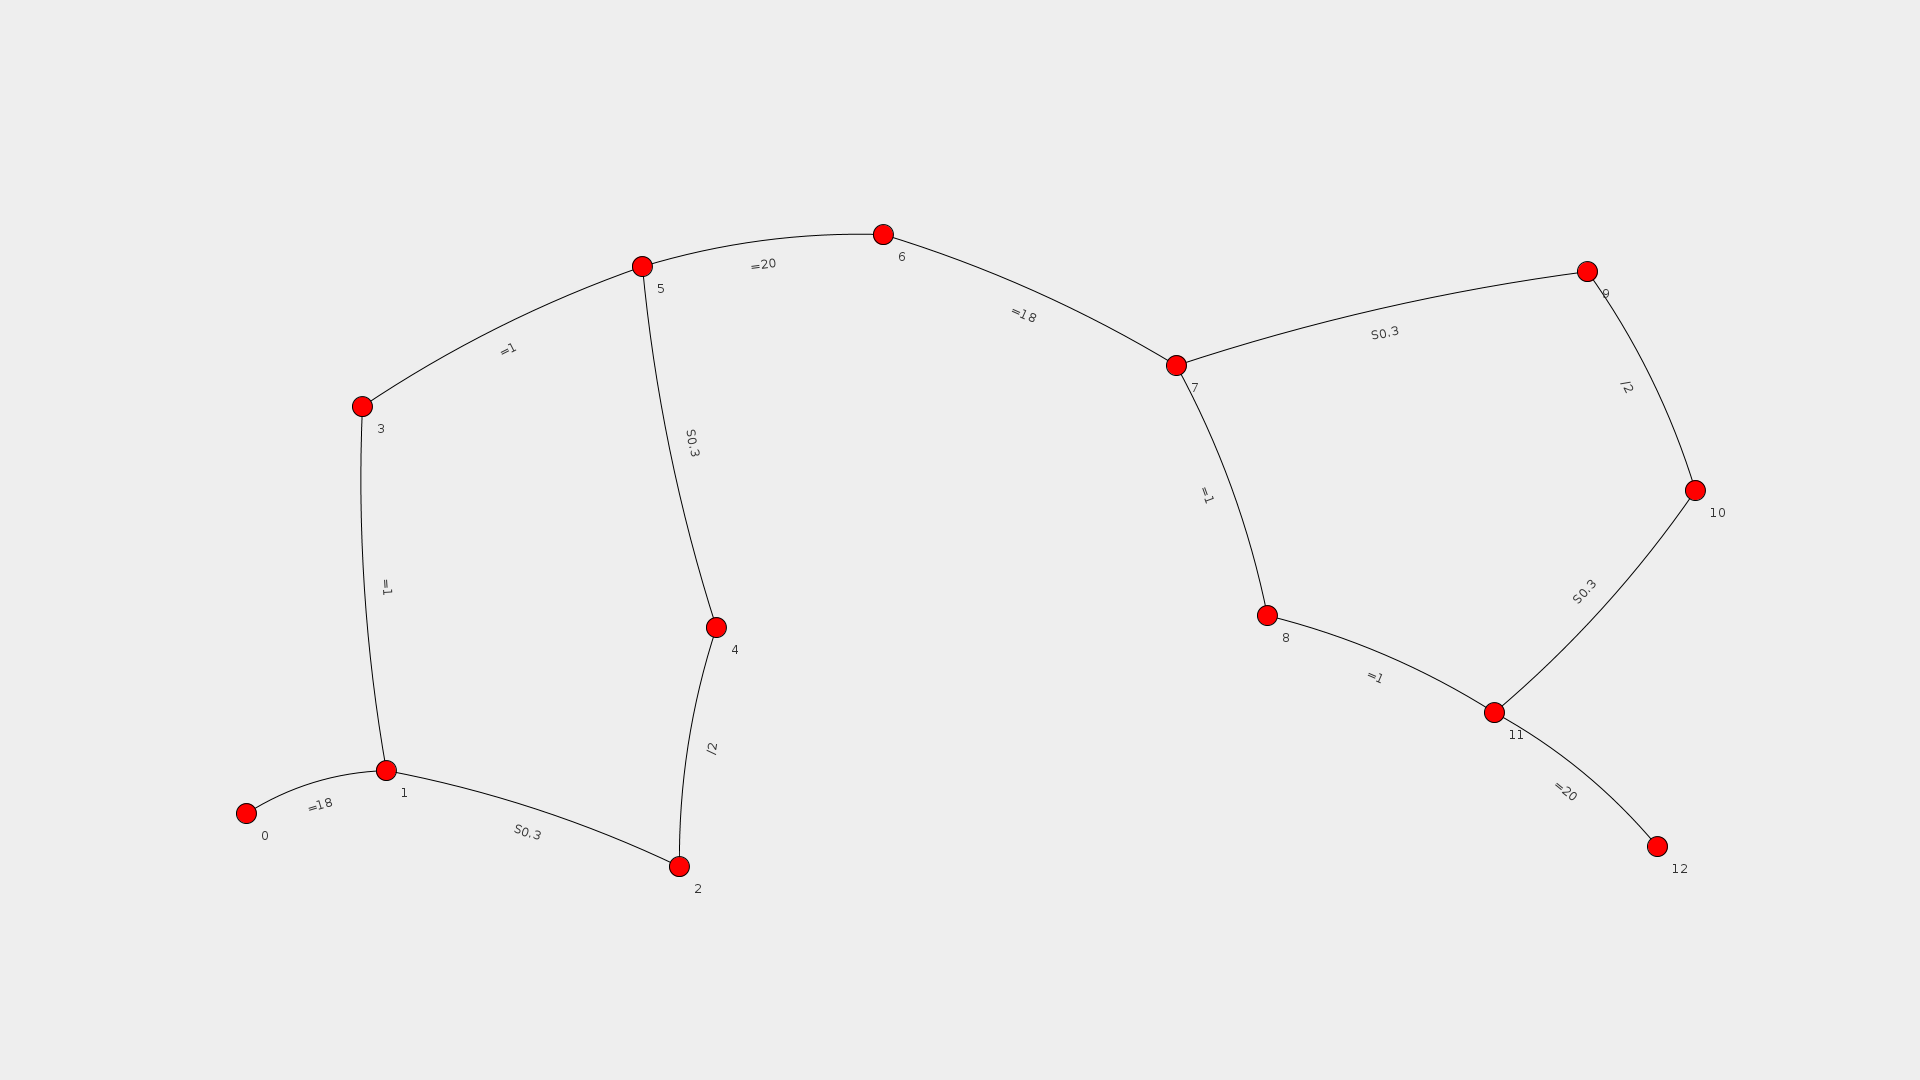
\includegraphics[width=150mm,angle=90]{solution.png}
\caption{RAS DATA SET TOY example territory. Undirected graph, arcs have descriptions.}
\end{figure}

\begin{figure}
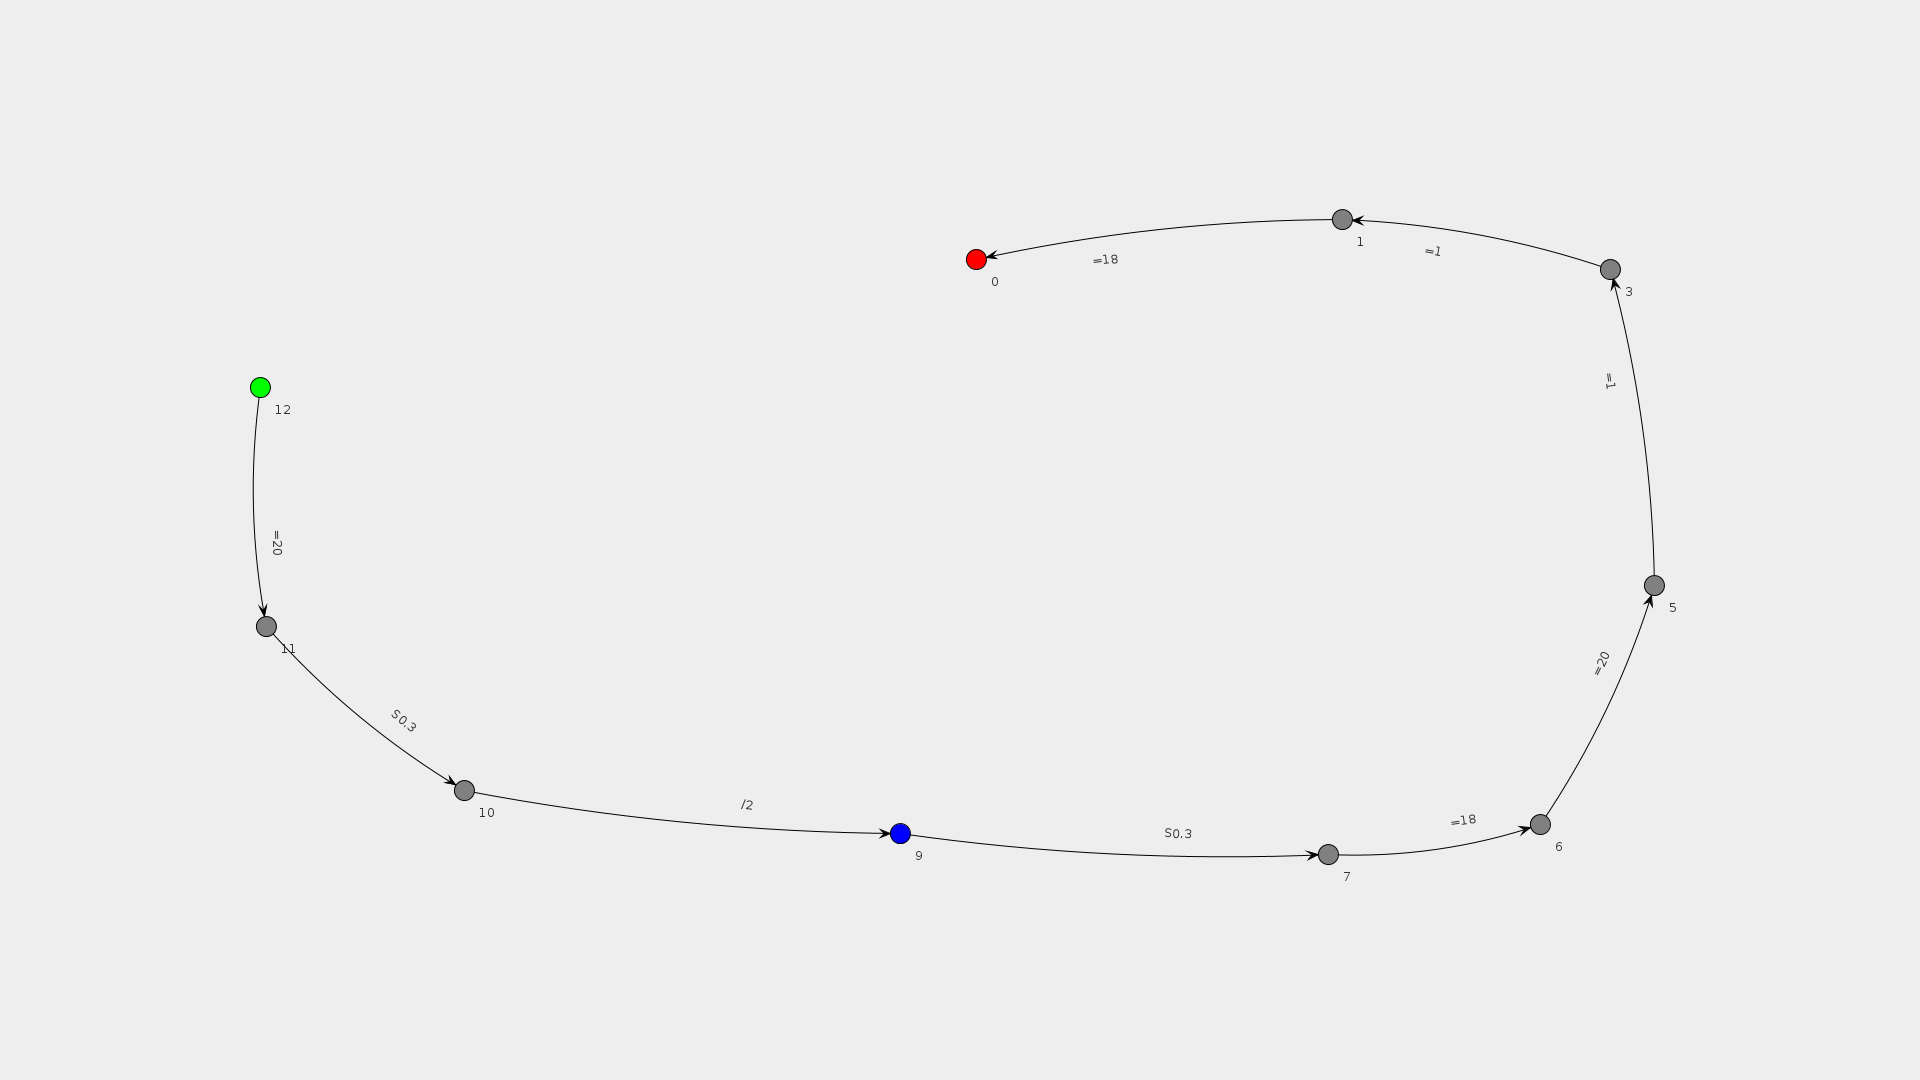
\includegraphics[width=150mm,angle=90]{B1.png}
\centering
\caption{RAS DATA SET TOY example, route of Train B1. Directed graph where green marks the origin, red the destination and blue is where the train is allowed to wait.}
\end{figure}

In this section, we show examples of visualizations that the solution is capable of providing. These visualizations have been rendered on the fly using the JUNG library\footnote{Java Universal Network/Graph framework, http://jung.sourceforge.net}.

\end{document}
